\documentclass[tikz,border=10pt]{standalone}
\usepackage{amsmath}
\begin{document}

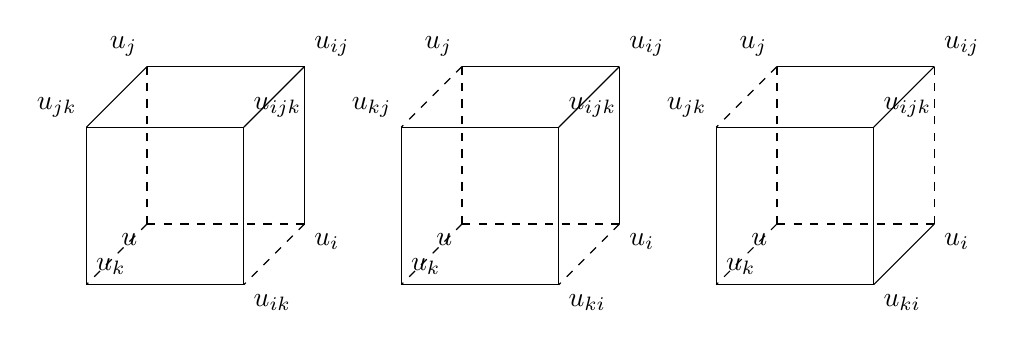
\begin{tikzpicture}
    % First cube
    \begin{scope}[scale=1]
        \coordinate (O) at (0,0,0);
        \coordinate (A) at (2,0,0);
        \coordinate (B) at (0,2,0);
        \coordinate (C) at (0,0,2);
        \coordinate (D) at (2,2,0);
        \coordinate (E) at (2,0,2);
        \coordinate (F) at (0,2,2);
        \coordinate (G) at (2,2,2);
        
        \draw[dashed] (O) -- (C);
        \draw[dashed] (O) -- (B);
        \draw[dashed] (O) -- (A);
        \draw[dashed] (A) -- (E);
        \draw (B) -- (D);
        \draw (C) -- (E);
        \draw (C) -- (F);
        \draw (B) -- (F);
        \draw (A) -- (D);
        \draw (E) -- (G);
        \draw (D) -- (G);
        \draw (F) -- (G);

        \node[below left] at (O) {$u$};
        \node[below right] at (A) {$u_i$};
        \node[above left] at (B) {$u_j$};
        \node[below right] at (E) {$u_{ik}$};
        \node[above right] at (D) {$u_{ij}$};
        \node[above left] at (F) {$u_{jk}$};
        \node[above right] at (G) {$u_{ijk}$};
        \node[above right] at (C) {$u_k$};
    \end{scope}
    
    % Second cube
    \begin{scope}[xshift=4cm, scale=1]
        \coordinate (O) at (0,0,0);
        \coordinate (A) at (2,0,0);
        \coordinate (B) at (0,2,0);
        \coordinate (C) at (0,0,2);
        \coordinate (D) at (2,2,0);
        \coordinate (E) at (2,0,2);
        \coordinate (F) at (0,2,2);
        \coordinate (G) at (2,2,2);
        
        \draw[dashed] (O) -- (C);
        \draw[dashed] (O) -- (B);
        \draw[dashed] (O) -- (A);
        \draw[dashed] (A) -- (E);
        \draw[dashed] (B) -- (F);
        \draw (C) -- (E);
        \draw (C) -- (F);
        \draw (B) -- (D);
        \draw (A) -- (D);
        \draw (E) -- (G);
        \draw (D) -- (G);
        \draw (F) -- (G);

        \node[below left] at (O) {$u$};
        \node[below right] at (A) {$u_i$};
        \node[above left] at (B) {$u_j$};
        \node[below right] at (E) {$u_{ki}$};
        \node[above right] at (D) {$u_{ij}$};
        \node[above left] at (F) {$u_{kj}$};
        \node[above right] at (G) {$u_{ijk}$};
        \node[above right] at (C) {$u_k$};
    \end{scope}
    
    % Third cube
    \begin{scope}[xshift=8cm, scale=1]
        \coordinate (O) at (0,0,0);
        \coordinate (A) at (2,0,0);
        \coordinate (B) at (0,2,0);
        \coordinate (C) at (0,0,2);
        \coordinate (D) at (2,2,0);
        \coordinate (E) at (2,0,2);
        \coordinate (F) at (0,2,2);
        \coordinate (G) at (2,2,2);
        
        \draw[dashed] (O) -- (C);
        \draw[dashed] (O) -- (B);
        \draw[dashed] (O) -- (A);
        \draw[dashed] (A) -- (D);
        \draw[dashed] (B) -- (F);
        \draw (C) -- (E);
        \draw (C) -- (F);
        \draw (B) -- (D);
        \draw (A) -- (E);
        \draw (E) -- (G);
        \draw (D) -- (G);
        \draw (F) -- (G);

        \node[below left] at (O) {$u$};
        \node[below right] at (A) {$u_i$};
        \node[above left] at (B) {$u_j$};
        \node[below right] at (E) {$u_{ki}$};
        \node[above right] at (D) {$u_{ij}$};
        \node[above left] at (F) {$u_{jk}$};
        \node[above right] at (G) {$u_{ijk}$};
        \node[above right] at (C) {$u_k$};
    \end{scope}
\end{tikzpicture}

\end{document}